\documentclass[../hydrozoa.tex]{subfiles}
\graphicspath{{\subfix{../images/}}}
\begin{document}

\chapter{L1 rule-based regime}%
\label{h:l1-rule-based-regime}%

If the peers stop responding to each other in the L2 consensus protocol, the L1~rule-based~regime ensures they can still withdraw their funds from the Hydrozoa head's treasury.
It is less cost-efficient and more complex than the multisig regime but serves as a fallback when L2 consensus breaks down.

The fallback from the multisig regime to the rule-based regime pins the L1 treasury's major version, disqualifying any L2 blocks with lesser or greater major versions.%
\footnote{Blocks with lesser major versions are disqualified because they assume a total treasury balance of funds that may no longer exist due to deposits and withdrawals adding/removing funds from the treasury.
  Blocks with greater major versions are disqualified because the fallback to the rule-based regime precludes their settlement transactions from being confirmed on L1 (utxo contention over the multisig treasury).}
The rule-based regime then proceeds via the following suite of Plutus scripts:
\begin{itemize}
  \item The dispute resolution scripts (\cref{h:l1-rule-based-dispute-resolution}) arbitrate the peers' dispute about the latest confirmed L2 block matching the L1 treasury's major version.
  \item The treasury spending validator (\cref{h:l1-rule-based-treasury}) awaits resolution and then manages withdrawals from the head's treasury based on the resolved L2 block.
\end{itemize}

The rule-based regime does not manage unabsorbed deposits left over from the multisig regime.
Depositors can retrieve them with post-dated refund transactions (\cref{h:l1-multisig-refund}) from the multisig regime.

\section{Utxo state}%
\label{h:l1-rule-based-utxo-state}%

In the rule-based regime, the head's L1 state resides in utxos at two different UPLC-script addresses:
\begin{equation*}
  \T{RuleBasedHeadState^{L1}} \coloneq \left\{
  \begin{array}{lll}
    \T{treasuryUtxo} &::& (\T{OutputRef}, \T{Output^{L1}}) \\
    \T{voteUtxos} &::& \T{UtxoSet^{L1}}
  \end{array}\right\}
\end{equation*}

\begin{figure}[H]
\begin{center}
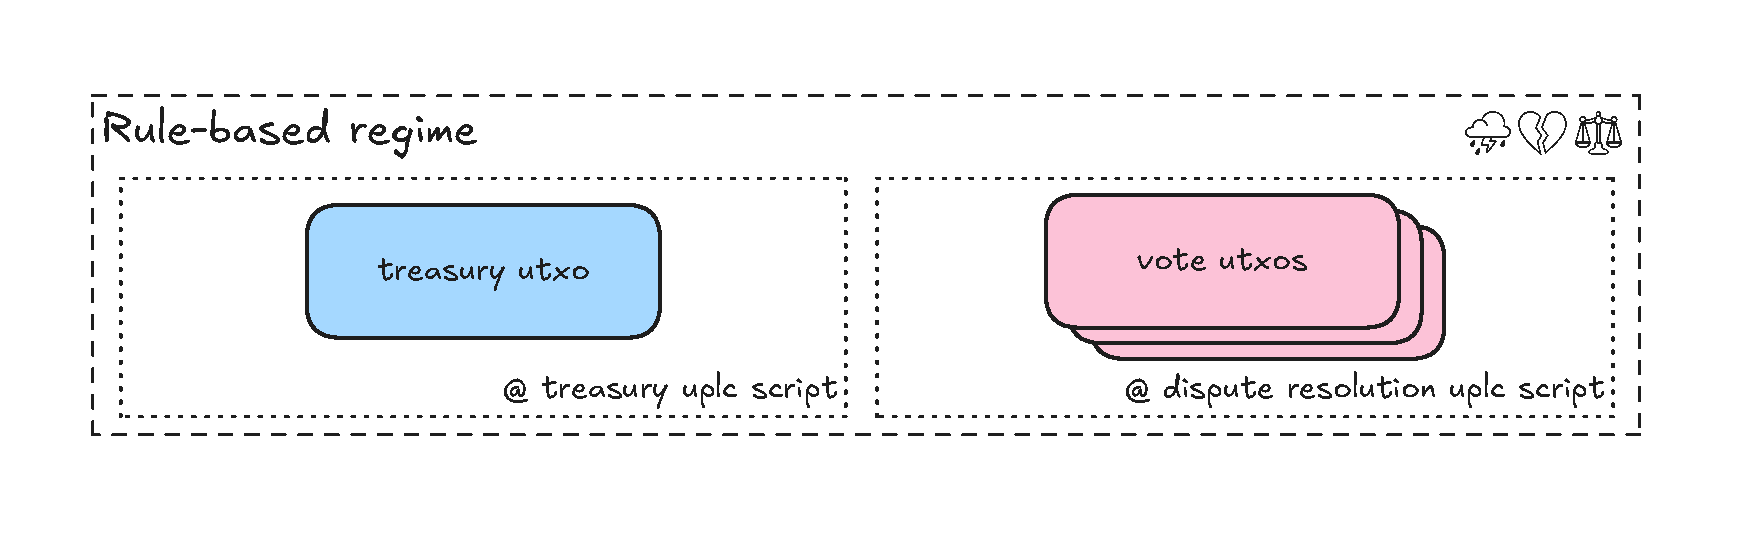
\includegraphics[width=\txDiagramScale\linewidth]{\subfix{../images/tx-diagram/1-rule-based-regime-utxo-state.pdf}}
\end{center}
\caption[Rule-based regime utxo state on L1.]{The L1 utxo state of the rule-based regime.}
\label{fig:utxo-state-rule-based-regime}
\end{figure}

\subsection{Treasury state}%
\label{h:l1-rule-based-treasury-state}%

In the rule-based regime, the head's treasury utxo is at the head's Plutus-based treasury address (\cref{h:l1-rule-based-treasury}).
It holds the head's beacon token and all treasury funds from the multisig regime (\cref{h:l1-multisig-utxo-state}).

The treasury utxo must have the following datum type, which defines its unresolved and resolved states in the rule-based regime:
\begin{equation*}
\begin{split}
  \T{RuleBasedTreasuryDatum} \coloneq&\;
    \T{Resolved} \; \T{ResolvedDatum} \\\mid&\;
    \T{Unresolved} \; \T{UnresolvedDatum} \\
  \T{ResolvedDatum} \coloneq&\;\left\{
    \begin{array}{lll}
      \T{headMp} &::& \T{PolicyId} \\
      \T{utxosActive}  &::& \mathcal{RH}_{32} \; \T{UtxoSet^{L2}} \\
      \T{version} &::& (\T{UInt}, \T{UInt}) \\
      \T{params} &::& \mathcal{H}_{32} \; \T{ParamsConsensusL2}
    \end{array}\right\} \\
  \T{UnresolvedDatum} \coloneq&\;\left\{
    \begin{array}{lll}
      \T{headMp} &::& \T{PolicyId} \\
      \T{disputeId} &::& \T{AssetName} \\
      \T{peers} &::& \T{[VerificationKey]} \\
      \T{peersN} &::& \T{UInt} \\
      \T{deadlineVoting} &::& \T{PosixTime} \\
      \T{versionMajor} &::& \T{UInt} \\
      \T{params} &::& \mathcal{H}_{32} \; \T{ParamsConsensusL2}
    \end{array}\right\}
\end{split}
\end{equation*}

The resolved treasury's datum is the same as the multisig treasury's datum, with these exceptions:
\begin{description}
  \item[head MP.] The policy ID of the head's native script minting policy.
  \item[version.] The full version of the resolved L2 block, which includes both the major and minor version numbers.
  It replaces the \code{versionMajor} field of the multisig treasury.
\end{description}

The unresolved treasury's datum fields are interpreted as follows:
\begin{description}
  \item[head MP.] The policy ID of the head's native script minting policy.
  \item[dispute ID.] The unique identifier used as the asset name of the dispute tokens (see below).
  \item[peers.] The peers' public keys.
  \item[n peers.] The number of peers in the head.
  \item[deadline voting.] A POSIX time before which votes can be cast in the dispute.
  \item[major version.] The treasury's major version, pinned by the fallback to the rule-based regime.
  \item[params.] A 32-byte Blake2b-256 hash (\codeMath{\mathcal{H}_{32}}) of the head's L2 consensus parameters (\cref{h:l2-head-state}).
\end{description}

\subsection{Dispute state}%
\label{h:l1-rule-based-dispute-state}%

Besides the treasury utxo, the head's state in the rule-based regime also includes the vote utxos for the dispute.
Each of these utxos is at the head's Plutus-based dispute address and holds one or more of the dispute's fungible tokens:
\begin{itemize}
  \item The policy ID corresponds to the head's native script (in minting policy form) (\cref{h:l1-multisig-regime}).
  \item The first four bytes of the asset name are equal to the CIP-67
    \citep{AlessandroKonradThomasVellekoopCIP67AssetName2022}
    prefix for class label \headDisputeToken{}, which corresponds to Hydrozoa head dispute tokens.%
    \footnote{We chose \headDisputeToken{} because it spells ``DISP'' (short for dispute) on a phone dial pad.}
  \item The last 28 bytes of the asset name are equal to the Blake2b-224 hash (\codeMath{\mathcal{H}_{28}}) of the multisig treasury utxo spent in the head's fallback to the rule-based regime (\cref{h:l1-rule-based-fallback}).
\end{itemize}

Each vote utxo has this datum type:
\begin{equation*}
\begin{split}
  \T{VoteDatum} &\coloneq \left\{
    \begin{array}{lll}
      \T{key}  &::& \T{UInt} \\
      \T{link} &::& \T{UInt} \\
      \T{peer} &::& \T{Maybe} \; \T{PubKeyHash} \\
      \T{voteStatus} &::& \T{VoteStatus}
    \end{array}\right\}\\
  \T{VoteStatus} &\coloneq \T{NoVote} \mid \T{Vote} \; \T{VoteDetails} \\
  \T{VoteDetails} &\coloneq \left\{
    \begin{array}{lll}
      \T{utxosActive} &::& \mathcal{RH}_{32} \; \T{UtxoSet^{L2}} \\
      \T{versionMinor} &::& \T{UInt}
    \end{array}\right\}
\end{split}
\end{equation*}

These fields are interpreted as follows:
\begin{description}
  \item[key.] An integer that uniquely identifies the vote utxo.
  \item[link.] An integer that uniquely references another vote utxo by its \code{key}.
  \item[peer.] The public-key hash of the peer (if any) who can cast a vote in this utxo.
  It is only empty for the default vote utxo (with \code{key} 0), which contains a vote that is automatically cast at the fallback to the rule-based regime (\cref{h:l1-rule-based-fallback}).
  \item[vote status.] Either no vote or a vote for a minor L2 block.
  \item[utxos active.] A 32-byte Merkle root hash (\codeMath{\mathcal{RH}_{32}}) of the L2 ledger's active utxo set, as of the block voted by the peer.
  \item[minor version.] The minor version of the minor L2 block voted by the peer.
  This block's major version must match the major version that the treasury had when it fell back to the rule-based regime.
\end{description}

Collectively, the vote utxos constitute a linked list data structure on L1.

\section{Fallback to rule-based regime}%
\label{h:l1-rule-based-fallback}%

The L2 consensus protocol pairs every multisig treasury utxo it creates with a post-dated fallback the treasury to the rule-based regime (\cref{h:l2-consensus-protocol}).

While L2 consensus holds, the peers store these post-dated transactions without submitting them.
However, if the multisig utxo is not spent by the time its corresponding post-dated transaction becomes valid, then L2 consensus is assumed to have stalled.
In that case, every peer should trigger the fallback to the rule-based regime by submitting the transaction to Cardano.

\begin{figure}[H]
\begin{center}
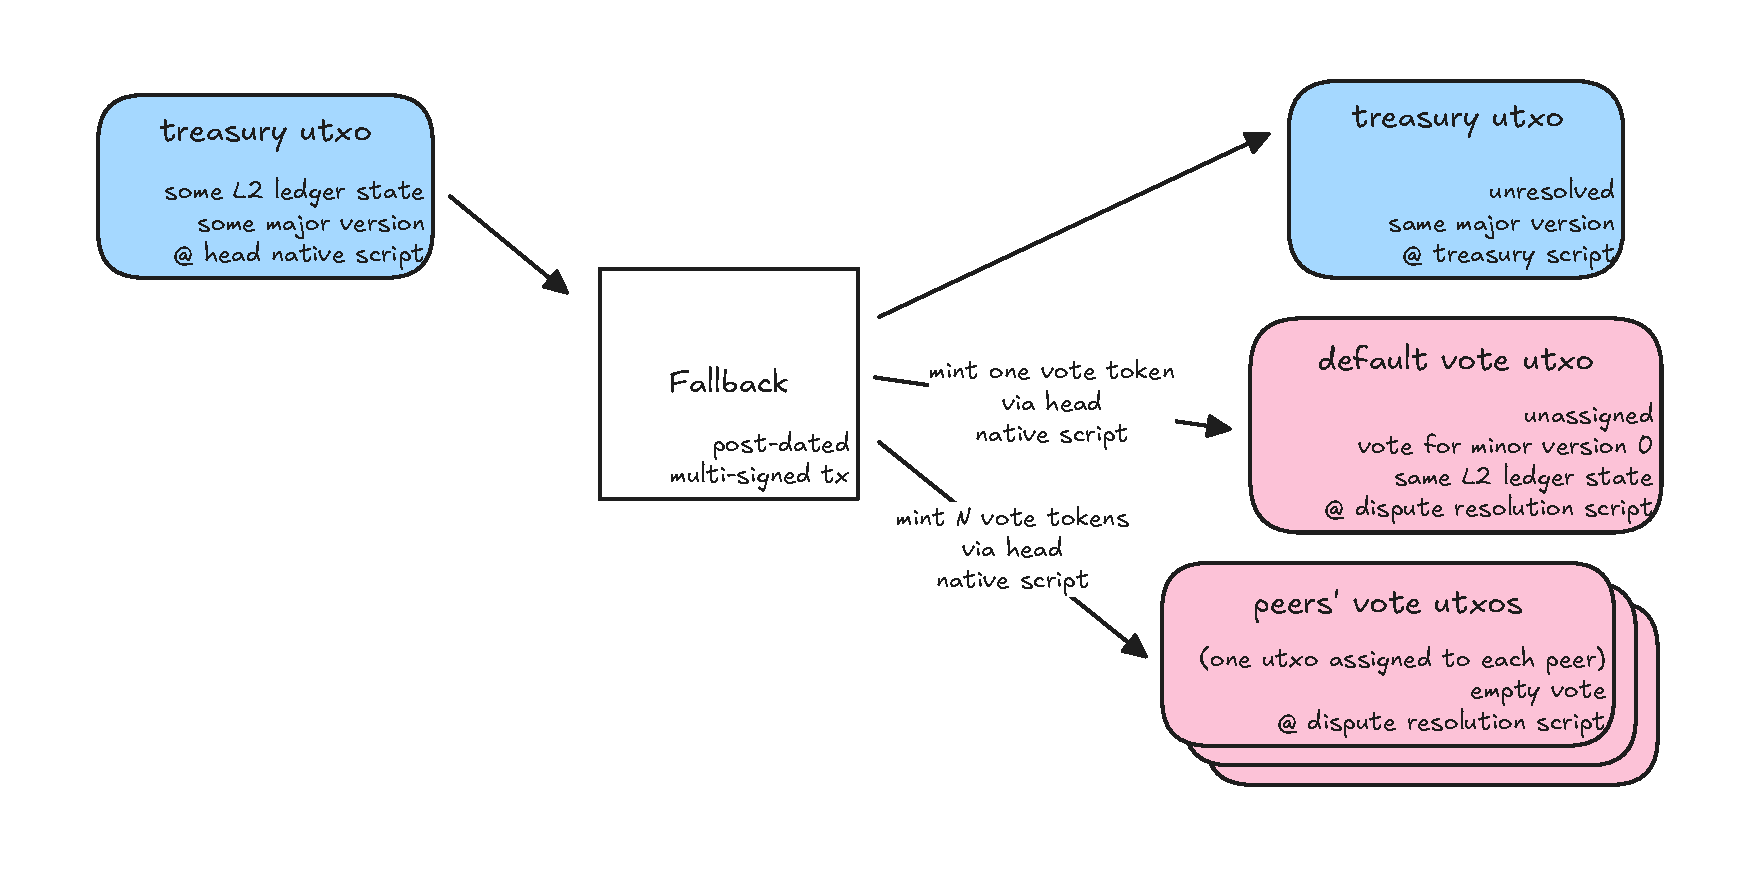
\includegraphics[width=\txDiagramScale\linewidth]{\subfix{../images/tx-diagram/8-fallback-tx.pdf}}
\end{center}
\caption[Rule-based regime: Fallback tx.]{The peers arrange for the head to fall back to the rule-based regime after a timeout, in case they fail to agree on any new settlement transactions to keep the multisig regime alive.}
\label{fig:tx-fallback}
\end{figure}

The transaction body is as follows:
\begin{enumerate}
  \item Spend the multisig treasury utxo (\code{multisigTreasury}).
    Let \code{mt} be its datum.
  \item Let \code{headMp} be the head's native script minting policy.
  \item Let \code{deadlineVoting} be the voting deadline for this dispute, as defined by the L2 consensus for this fallback to the rule-based regime.
  \item Let \code{disputeId} be the CIP-67 prefix for 3477, concatenated with the Blake2b-224 hash (\codeMath{\mathcal{H}_{28}}) of the \code{multisigTreasury} output reference.
  \item Let \code{peers} be a list of the peers' public keys and \code{peersN} be its length.%
    \footnote{The indices of the \code{peers} list (and all other lists in this specification) start from \inlineColored{1}.}
  \item Mint (\code{peersN} + 1) dispute tokens of (\code{headMp}, \code{disputeId}).
  \item Create the rule-based treasury utxo (\code{ruleBasedTreasury}), containing the funds and beacon token from \code{multisigTreasury} and this datum:
    \begin{equation*}
    \begin{split}
      \T{FallbackTreasuryDatum} \coloneq \T{Unresolved} \;\left\{
        \begin{array}{lll}
          \T{headMp} &=& \T{headMp} \\
          \T{disputeId} &=& \T{disputeId} \\
          \T{peers} &=& \T{peers} \\
          \T{peersN} &=& \T{peersN} \\
          \T{deadlineVoting} &=& \T{deadlineVoting} \\
          \T{versionMajor} &=& \T{mt.majorVersion} \\
          \T{params} &=& \T{mt.params}
        \end{array}\right\}
    \end{split}
    \end{equation*}
  \item Create the default vote utxo, containing a vote for the major L2 block's active utxo set:
    \begin{equation*}
      \T{defaultVoteDatum} \coloneq \left\{
      \begin{array}{lll}
        \T{key} &=& 0 \\
        \T{link} &=& 0 < \T{peersN} \;?\; 1 : 0 \\
        \T{peer} &=& \T{Nothing} \\
        \T{voteStatus} &=& \T{Vote} \left\{
        \begin{array}{lll}
            \T{utxosActive} &=& \T{mt.utxosActive} \\
            \T{versionMinor} &=& 0
        \end{array}\right\}
      \end{array}\right\}
    \end{equation*}
  \item For \codeMath{i} iterated from 1 to \code{peersN}, create a vote utxo with one dispute token and this datum:%
    \begin{equation*}
      \T{initVoteDatum} \; i \coloneq \left\{
        \begin{array}{lll}
          \T{key}  &=& i \\
          \T{link} &=& i < \T{peersN} \;?\; (i + 1) : 0 \\
          \T{peer} &=& \T{Just} \; (\mathcal{H}_{32} \; \T{peers}[i]) \\
          \T{voteStatus} &=& \T{NoVote}
        \end{array}\right\}\\
    \end{equation*}
\end{enumerate}

\section{Dispute resolution}%
\label{h:l1-rule-based-dispute-resolution}%

During the voting period of a dispute, each peer gets one opportunity to cast their vote on the latest minor L2 block confirmed by the L2 consensus protocol before it stalled.
When all votes are cast or the voting period ends, the dispute's state can be resolved to a single vote utxo containing the latest block among the votes.

Voting is handled by the Plutus-based spending validator of the dispute address.
We describe its redeemers in the rest of this section.

\subsection{Vote}%
\label{h:l1-dispute-resolution-vote-redeemer}%

\begin{figure}[H]
\begin{center}
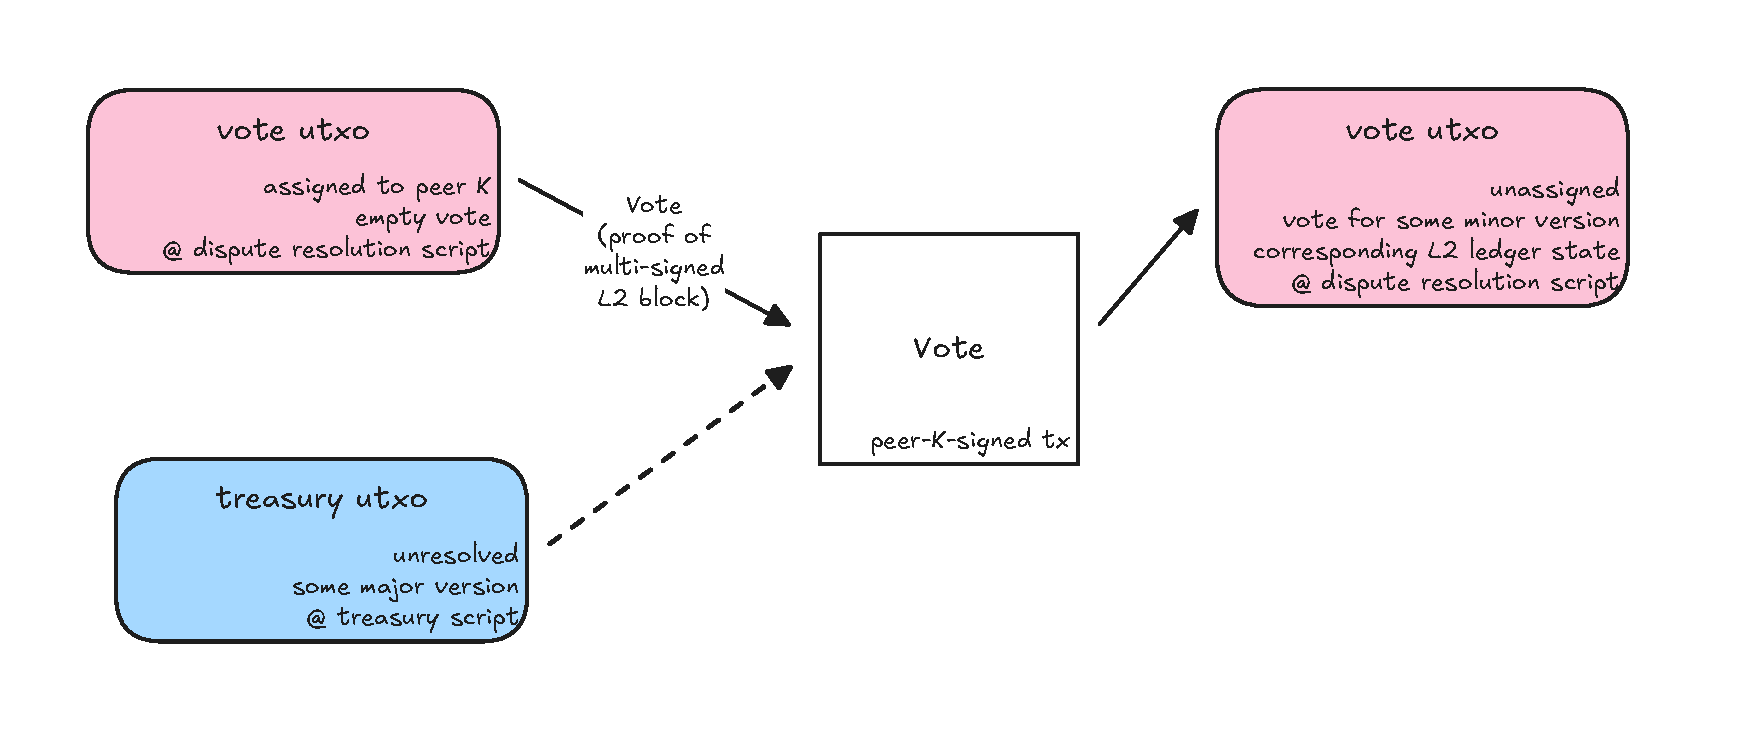
\includegraphics[width=\txDiagramScale\linewidth]{\subfix{../images/tx-diagram/9-vote-tx.pdf}}
\end{center}
\caption[Rule-based regime: Vote tx.]{A peer casts its vote for the latest confirmed L2 block version from the multisig regime.}
\label{fig:tx-vote}
\end{figure}

Replace the input's no-vote status with an abstention or a valid vote for a block.
Conditions:
\begin{itemize}
  \item Verify the vote inputs:
    \begin{enumerate}
      \item Let \code{voteOutref} be the output reference of the input being spent.
      \item Let \code{voteInput} be the input being spent.
        There must not be any other spent input matching \code{voteOutref} on transaction hash.
      \item The \code{voteStatus} field of \code{voteInput} must be \code{NoVote}.
      \item The transaction must be signed by the \code{peer} field of \code{voteInput}, if it is non-empty.
      \item Let (\code{headMp}, \code{disputeId}) be the minting policy and asset name of the only non-ADA tokens in \code{voteInput}.
    \end{enumerate}
  \item Verify the treasury reference input:
    \begin{enumerate}[resume]
      \item Let \code{treasury} be the only reference input matching \code{voteOutref} on tx hash.
      \item A head beacon token of \code{headMp} and CIP-67 prefix \headBeaconToken{} must be in \code{treasury}.
      \item \code{headMp} and \code{disputeId} must match the corresponding fields of the \code{Unresolved} datum in \code{treasury}.
      \item The transaction's time-validity upper bound must not exceed the \code{deadlineVoting} field of \code{treasury}.
    \end{enumerate}
  \item Verify the redeemer:
    \begin{enumerate}[resume]
      \item Let \code{voteRedeemer} be an \emph{optional} redeemer argument with this type:%
        \footnote{These types are defined in \cref{h:l2-blocks} and repeated here.}
        \begin{equation*}
        \begin{split}
          \T{MinorBlockL1Effect} &\coloneq \left\{
            \begin{array}{lll}
              \T{blockHeader} &::& \T{BlockHeader^{L2}} \\
              \T{multisig} &::& [\T{Signature}]
            \end{array}\right\}\\
          \blockHeaderTypeName{} &\coloneq \blockHeaderTypeBody{}
        \end{split}
        \end{equation*}
      \item If \code{voteRedeemer} is provided, then both of these must hold:
        \begin{enumerate}
          \item The \code{multisig} field of \code{voteRedeemer} must have signatures of the \code{blockHeader} field of \code{voteRedeemer} for all the public keys in the \code{peers} field of \code{treasury}.
          \item The \code{versionMajor} field must match between \code{treasury} and \code{voteRedeemer}.
        \end{enumerate}
    \end{enumerate}
  \item Verify the vote output:
    \begin{enumerate}[resume]
      \item Let \code{voteOutput} be an output with the same number of (\code{headMp}, \code{disputeId}) tokens and same address as \code{voteInput}.
      It must not hold any other non-ADA tokens.
      \item If \code{voteRedeemer} is provided, the \code{voteStatus} field of \code{voteOutput} must be a \code{Vote} matching \code{voteRedeemer} on the \code{utxosActive} and \code{versionMinor} fields.
      \item All other fields of \code{voteInput} and \code{voteOutput} must match.
    \end{enumerate}
\end{itemize}

\subsection{Tally}%
\label{h:l1-dispute-resolution-tally-redeemer}%

\begin{figure}[H]
\begin{center}
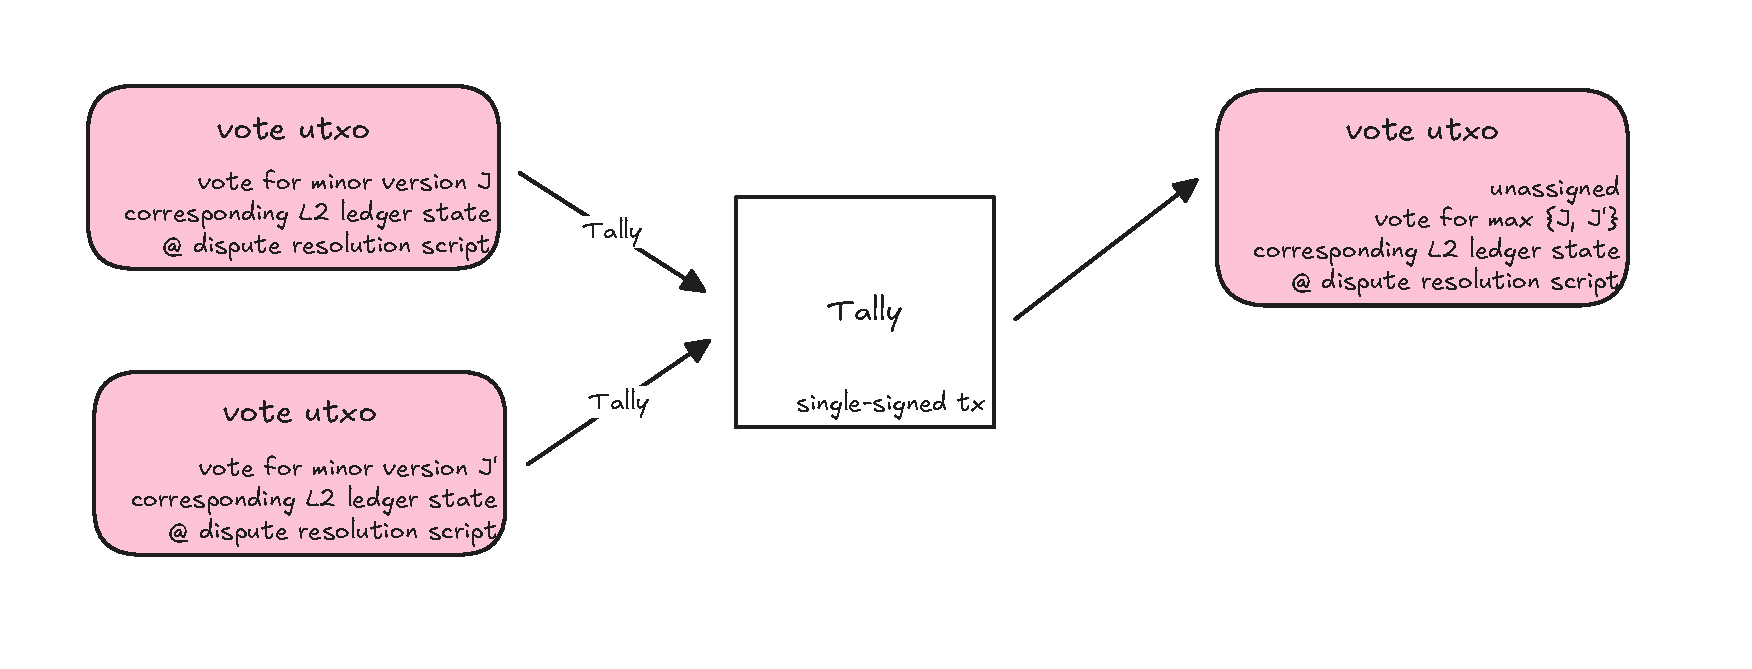
\includegraphics[width=\txDiagramScale\linewidth]{\subfix{../images/tx-diagram/A-tally-tx.pdf}}
\end{center}
\caption[Rule-based regime: Tally tx.]{Collapse two votes into one, keeping the latest confirmed L2 block version among them.}
\label{fig:tx-tally}
\end{figure}

Collapse two votes into one, keeping the latest confirmed L2 block version among them.
Conditions:
\begin{itemize}
  \item Verify the vote inputs:
    \begin{enumerate}
      \item Let \code{tallyRedeemer} be a redeemer argument with this type:
        \begin{equation*}
          \T{TallyRedeemer} \coloneq \left\{
          \begin{array}{lll}
            \T{continuingOutref} &::& \T{OutputRef} \\
            \T{removedOutref} &::& \T{OutputRef}
          \end{array}\right\}
        \end{equation*}
      \item Let \code{continuingInput} and \code{removedInput} be spent inputs with the respective output references of \code{tallyRedeemer}.
      \item \code{continuingInput} and \code{removedInput} must match on address.
      \item \code{continuingInput} and \code{removedInput} must have non-ADA tokens of only one asset class, which must match between them and satisfy both of the following:
        \begin{enumerate}
          \item The minting policy (\code{headMp}) must be a native script.
          \item The asset name (\code{disputeId}) must have the CIP-67 prefix \headDisputeToken{}.
        \end{enumerate}
      \item The \code{key} field of \code{removedInput} must be greater than the \code{key} field and equal to the \code{link} field of \code{continuingInput}.
      \item There must be no other spent inputs from the same address as \code{continuingInput} or holding any tokens of \code{headMp}.
    \end{enumerate}
  \item Verify the treasury reference input:
    \begin{enumerate}[resume]
      \item If the \code{voteStatus} of either \code{continuingInput} or \code{removedInput} is \code{NoVote}, all of the following must be satisfied:
        \begin{enumerate}
          \item Let \code{treasury} be a reference input holding the head beacon token of \code{headMp} and CIP-67 prefix \headBeaconToken{}.
          \item \code{headMp} and \code{disputeId} must match the corresponding fields of the \code{Unresolved} datum in \code{treasury}.
          \item The \code{deadlineVoting} field of \code{treasury} must not exceed the transaction's time-validity lower bound.
        \end{enumerate}
    \end{enumerate}
  \item Verify the vote output:
    \begin{enumerate}[resume]
      \item Let \code{continuingOutput} be an output with the same address and the sum of all tokens (including ADA) in \code{continuingInput} and \code{removedInput}.
      \item The \code{voteStatus} field of \code{continuingOutput} must match the highest \code{voteStatus} of \code{continuingInput} and \code{removedInput}, totally ordered as follows:
        \begin{equation*}
        \begin{split}
          &\forall a, b \in \T{VoteDetails}:\\
          &\quad a \T{.minorVersion} \leq b \T{.minorVersion} \implies\\
          &\qquad \T{NoVote} < \T{Vote} \; a \leq \T{Vote} \; b  
        \end{split}
        \end{equation*}
      \item The \code{link} field of \code{removedInput} and \code{continuingOutput} must match.
      \item All other fields of \code{continuingInput} and \code{continuingOutput} must match.
    \end{enumerate}
\end{itemize}

\subsection{Resolve}%
\label{h:l1-dispute-resolution-resolve-redeemer}%

The sole remaining vote utxo can be spent when the treasury utxo is spent.
Conditions:
\begin{enumerate}
  \item Let \code{voteInput} be the input being spent.
  \item Let (\code{headMp}, \code{disputeId}) be the minting policy and asset name of the only non-ADA tokens in \code{voteInput}.
  \item Let \code{treasury} be a spent input that holds a head beacon token of \code{headMp} and CIP-67 prefix \headBeaconToken{}.
  \item \code{headMp} and \code{disputeId} must match the corresponding fields of the \code{Unresolved} datum in \code{treasury}.
\end{enumerate}

\section{Treasury}%
\label{h:l1-rule-based-treasury}%

The treasury spending validator awaits the dispute's resolution and adopts the active utxo set of the resolved L2 block.
Peers can then withdraw funds from the treasury by creating utxos on L1 and showing Merkle proofs of equivalent utxos being removed from the treasury's active utxo set.

We describe the treasury spending validator's redeemers in the rest of this section.

\subsection{Resolve}%
\label{h:l1-treasury-resolve-redeemer}%

\begin{figure}[H]
\begin{center}
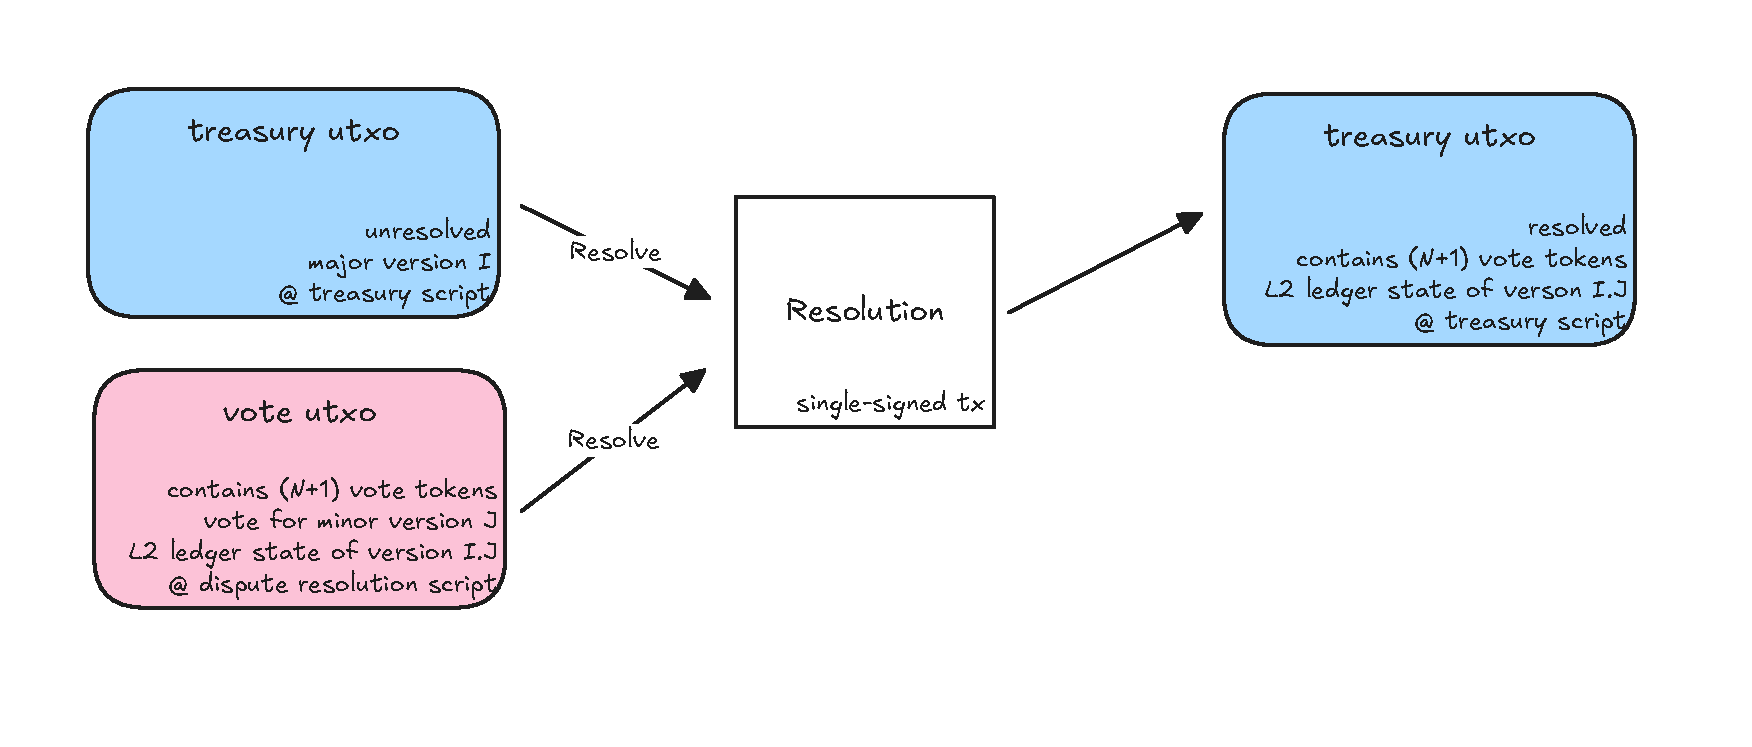
\includegraphics[width=\txDiagramScale\linewidth]{\subfix{../images/tx-diagram/B-resolution-tx.pdf}}
\end{center}
\caption[Rule-based regime: Resolution tx.]{Resolve the peers' dispute by applying the latest confirmed L2 block to the treasury utxo.
Funds will now be withdrawable based on that block's L2 ledger state.}
\label{fig:tx-resolution}
\end{figure}

Resolve the treasury's state based on the sole remaining vote utxo.
Conditions:
\begin{enumerate}
  \item Let \code{treasuryInput} be the input being spent.
  \item Let \code{headMp}, \code{disputeId}, \code{peersN}, and \code{versionMajor} be the corresponding fields of \code{treasuryInput}.
  \item Let \code{voteInput} be a spent input with (\code{peersN} + 1) tokens of (\code{headMp}, \code{disputeId}) and no other non-ADA tokens.
  \item Let \code{treasuryOutput} be an output with the same address as \code{treasuryInput} and the sum of all tokens (including ADA) in \code{treasuryInput} and \code{voteInput}.
  \item Let \code{voteStatus} be the corresponding field of \code{voteInput}. \code{voteStatus} must be \code{Vote}.
  \item Let \code{versionMinor} be the corresponding field in \code{voteStatus}.
  \item The \code{version} field of \code{treasuryOutput} must match (\code{versionMajor}, \code{versionMinor}).
  \item \code{voteStatus} and \code{treasuryOutput} must match on \code{utxosActive}.
  \item \code{treasuryInput} and \code{treasuryOutput} must match on all other fields.
\end{enumerate}

\subsection{Withdraw}%
\label{h:l1-treasury-withdraw-redeemer}%

\begin{figure}[H]
\begin{center}
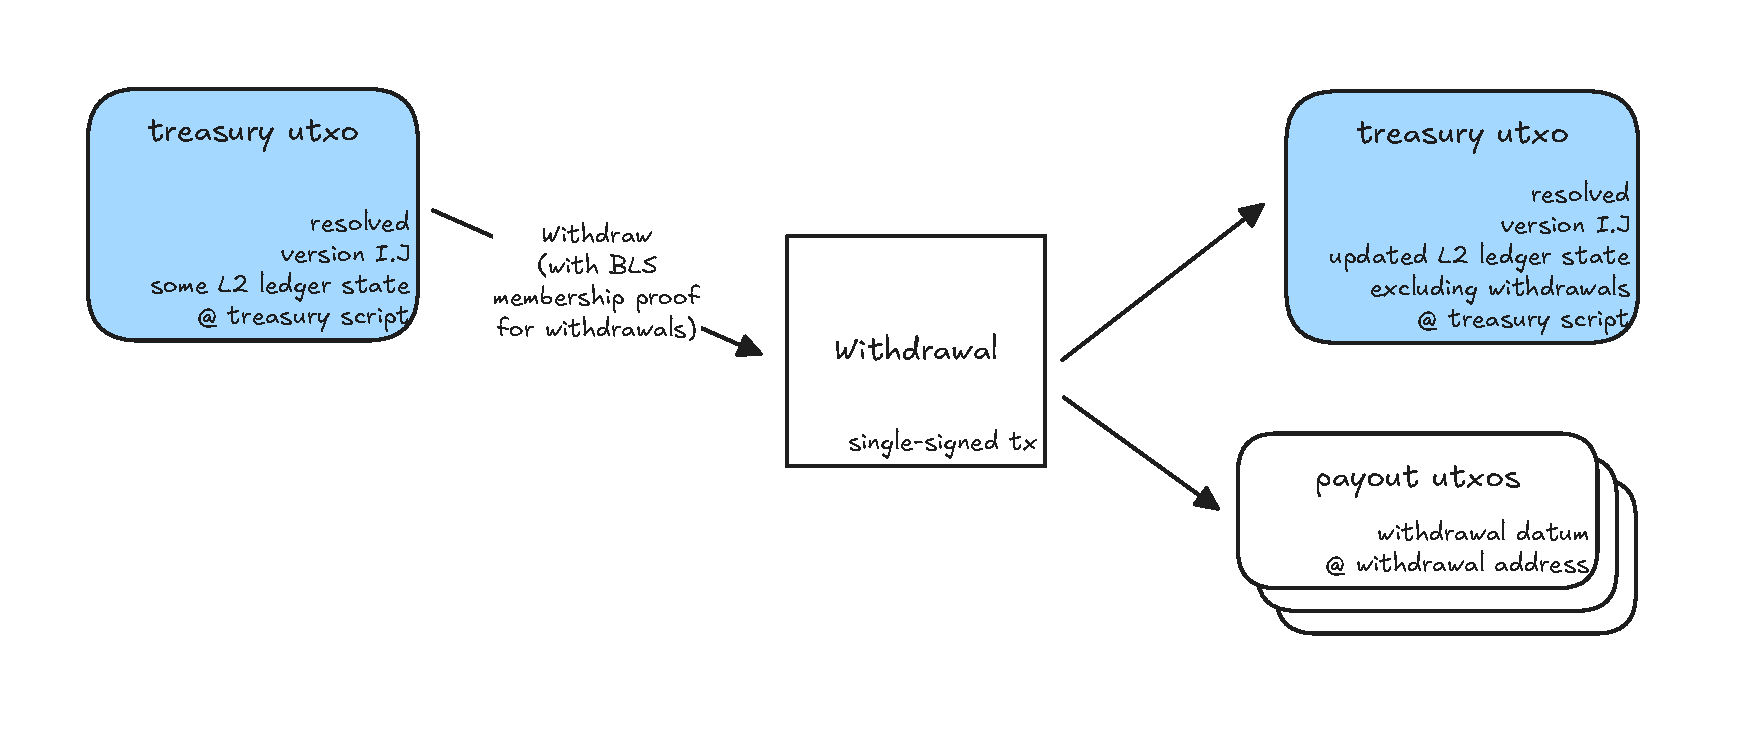
\includegraphics[width=\txDiagramScale\linewidth]{\subfix{../images/tx-diagram/C-withdrawal-tx.pdf}}
\end{center}
\caption[Rule-based regime: Withdrawal tx.]{Withdraw funds from the treasury via membership proof of utxos in the resolved L2 ledger state.
Update the resolved L2 ledger state to exclude those utxos.}
\label{fig:tx-withdrawal}
\end{figure}

Withdraw treasury funds and update its active utxo set accordingly.
Conditions:
\begin{enumerate}
  \item Let \code{treasuryInput} be the input being spent.
  \item Let \code{headMp} be the corresponding field in \code{treasuryInput}.
  \item Let \code{headId} be the asset name of the only \code{headMp} token in \code{treasuryInput} with CIP-67 prefix \headBeaconToken{}.
  \item Let \code{withdrawals} be a list of triples provided as a redeemer argument.
      Each triple contains an output reference, an L2 output, and a Merkle inclusion proof.
      The proof shows a path from some Merkle root hash to the L2 output at the output reference.
      \begin{equation*}
        \left[\left(
          \T{OutputRef},\;
          \T{Output^{L2}},\;
          \T{MerkleProof}
        \right)\right]
      \end{equation*}
  \item Let \code{treasuryOutput} be the first transaction output. It must hold the (\code{headMp}, \code{headId}) beacon token.
  \item Let \code{outputsRemaining} be a mutable variable initialized to the transaction's outputs, excluding \code{treasuryOutput}.
  \item Let \code{valueTotal} be a mutable variable initialized to the value of \code{treasuryOutput}.
  \item Let \code{rootHash} be a mutable variable initialized to the \code{utxosActive} of \code{treasuryInput}.
  \item For each triple \codeMath{(\T{outref}, \T{outputL2}, \T{proof})} in \code{withdrawals}:
    \begin{enumerate}
      \item Let \code{outputL1} be the first element in \code{outputsRemaining}, which must exist.
      \item \code{outputL1} and \code{outputL2} must match on the \code{value}, \code{datum}, and \code{script} fields.
      \item \code{outputL1} and \code{outputL2} must match on the \code{addr} field by payment credential and staking reference.
      \item Update \code{outputsRemaining} by excluding \code{outputL1}.
      \item Update \code{valueTotal} by adding the value of \code{outputL1}.
      \item Update \code{rootHash} by applying the Merkle library's \code{delete} function with the triple:
        \begin{equation*}
          \T{delete} ::
            \mathcal{RH}_{32} \; \T{UtxoSet^{L2}} ->
            (\T{OutputRef}, \T{Output^{L2}}, \T{Proof}) ->
            \mathcal{RH}_{32} \; \T{UtxoSet^{L2}}
        \end{equation*}
    \end{enumerate}
  \item \code{valueTotal} must match the value of \code{treasuryInput}.
  \item \code{rootHash} must match the \code{utxosActive} of \code{treasuryOutput}.
\end{enumerate}

\subsection{Deinit}%
\label{h:l1-treasury-deinit}%

\begin{figure}[H]
\begin{center}
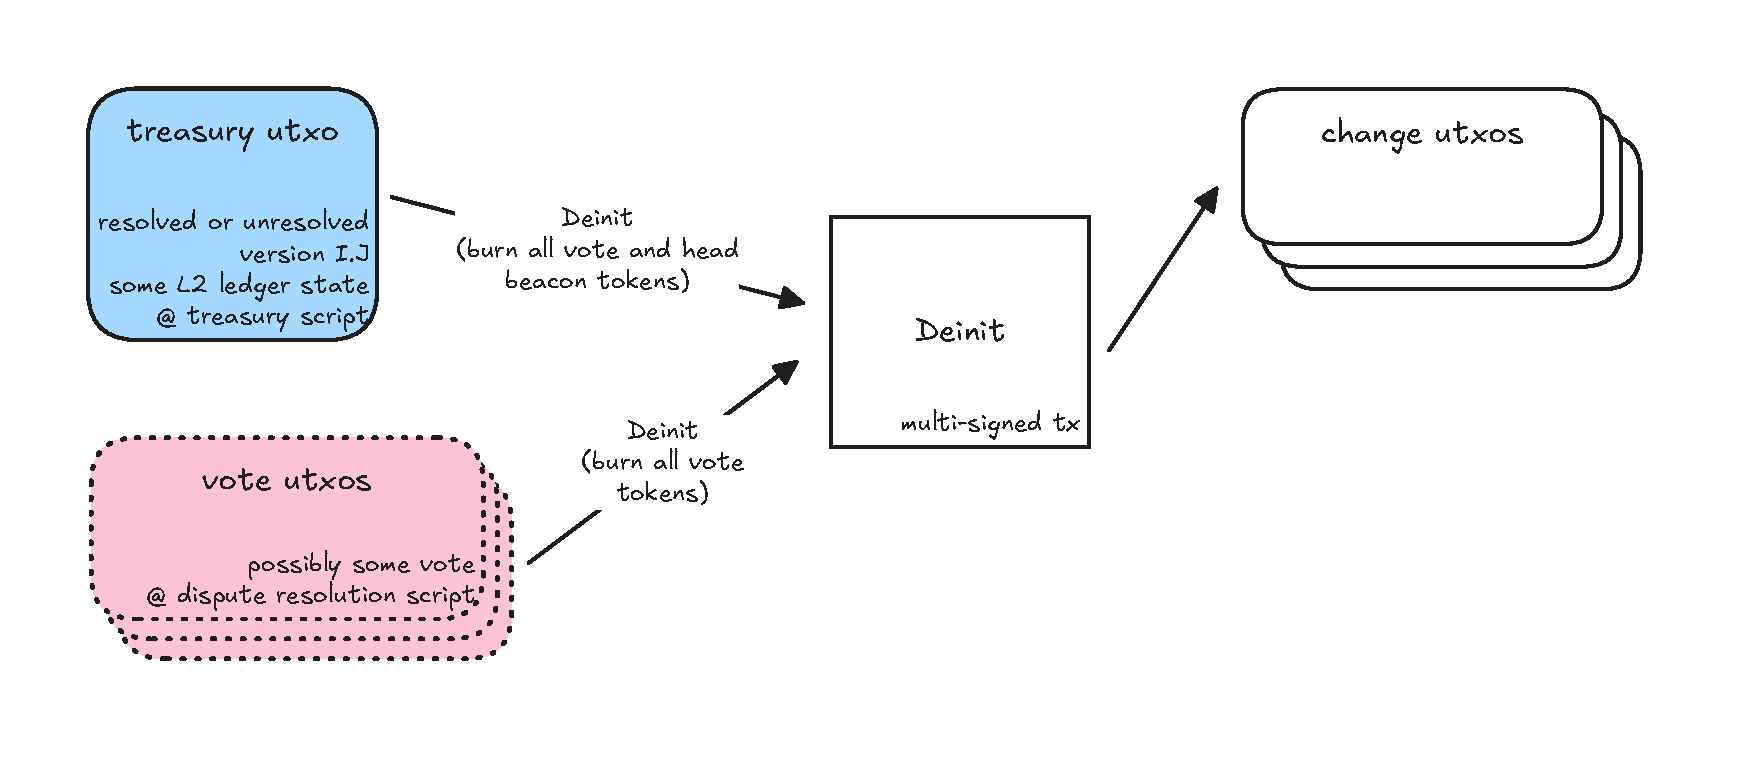
\includegraphics[width=\txDiagramScale\linewidth]{\subfix{../images/tx-diagram/D-deinit-tx.pdf}}
\end{center}
\caption[Rule-based regime: de-initialization tx.]{The peers deinitialize the head's treasury and clean-up any remnants of head state.}
\label{fig:tx-deinit}
\end{figure}

De-initialize the head, removing all traces of it.
Conditions:%
\footnote{This redeemer does not require the treasury's active utxo set to be empty, but it implicitly requires the transaction to be multi-signed by all peers to burn the \inlineColored{headMp} tokens.
  Thus, the peers can use this redeemer to override the treasury's spending validator with their multi-signature.}
\begin{enumerate}
  \item Let \code{treasury} be the input being spent.
  \item Let \code{headMp} be the corresponding field in \code{treasury}.
  \item All \code{headMp} tokens in \code{treasury} with CIP-67 prefixes of \headDisputeToken{} and \headBeaconToken{} must be burned.
\end{enumerate}

\end{document}
